\chapter{뉴턴 우주론과 프리드만 방정식}

지난 시간에는 공간의 계량에 관해 이야기했습니다. 다음 질문은 동역학입니다. 스케일 인자는 시간에 따라 어떻게 변할까요? 먼저 간단한 기하학을 살펴본 뒤 뉴턴 우주론으로 넘어가겠습니다. 여기서는 일반 상대성 이론으로부터 프리드만 방정식을 유도하지 않습니다. 뉴턴 방정식으로 유도하겠습니다.

\section{균질성, 등방성과 시간에 따라 변하는 계량}

균질성과 등방성을 기본 가정으로 둡니다. 우주가 균질하고 등방적이며 시간에 따라 변한다면 허블 법칙은 언제나 성립합니다. 어느 한 시각을 고정하면 후퇴 속도는 거리에 비례합니다.
\begin{equation}
v = H(t)\,d.
\end{equation}
비례 관계는 선형입니다. 일정한 것은 시간이 아니라 공간입니다. 주어진 순간에는 어디에서나 같은 비례 상수가 적용됩니다.

\begin{classroomqa}
\audiencequestion{선형 비례한다는 뜻인가요?}\lecturetimestamp{00:02:06}
\lecturerresponse{그렇습니다. 시각을 고정하면 후퇴 속도는 거리에 선형 비례합니다. 비례 상수가 허블 상수입니다. 일반적으로 이 값은 시간에 따라 달라지지만 공간상의 위치에 따라 달라지지는 않습니다.}
\end{classroomqa}

그래서 ``허블 상수''라는 표현은 주의해서 써야 합니다. 공간상의 위치에 대해서는 상수입니다. 시간에 대해서는 상수가 아닙니다.

자연스럽게 이런 질문이 나옵니다. 공간이 팽창한다면 왜 미터 자도 함께 늘어나지 않을까요? 원자 규모에서 미터 자를 결속하는 힘은 우주 팽창과 관련된 어떤 효과보다도 압도적으로 강하기 때문입니다. 결합된 물체는 결합된 상태를 유지합니다. 팽창하는 것은 충분히 떨어져 있어 서로 강하게 붙잡고 있지 않은 은하들 사이의 거리입니다.

\begin{classroomqa}
\audiencequestion{측정용 자도 함께 팽창한다는 사실은 문제가 되지 않나요?}\lecturetimestamp{00:04:00}
\lecturerresponse{아닙니다. 측정용 자는 팽창하지 않습니다. 팽창하는 것은 좌표입니다. 미터 자를 결속하는 힘은 팽창에 따른 효과보다 훨씬 강하므로, 보통의 결합된 물체는 배경과 함께 팽창하지 않습니다. 충분히 멀리 떨어진 은하들은 서로 멀어지지만 미터 자는 그렇지 않습니다.}
\end{classroomqa}

원자 사이에 아주 작은 추가적인 척력 효과가 있다고 상상해 볼 수도 있습니다. 그래도 막대를 잡아당겨 부러뜨리지는 못합니다. 단지 평형 간격을 조금 바꿀 뿐입니다. 작은 추가 힘이 단단한 용수철의 평형 위치를 약간 바꾸는 것과 같습니다.

\begin{classroomqa}
\audiencequestion{그렇지만 점들 사이의 힘으로 모델링할 수는 없는 거죠? 그렇지 않으면 가속도가 생길 테니까요.}\lecturetimestamp{00:05:29}
\lecturerresponse{원자 사이에 작은 추가 힘이 있다고 상상할 수는 있습니다. 다만 그 힘이 결합력에 비해 아주 작다면 평형 위치만 조금 바뀝니다. 팽창 자체가 보통의 힘 법칙을 만들어 내지는 않습니다. 일부 팽창은 힘으로 모델링할 수 있는데, 가속 팽창이 그 예입니다. 하지만 그것은 나중에 다룰 문제입니다.}
\end{classroomqa}

따라서 유용한 좌표는 팽창하는 물질 분포에 붙어 있는 좌표입니다. 별도의 특이 속도가 없는 은하들은 같은 좌표값을 유지합니다. 시간에 따라 변하는 것은 좌표 간격과 미터 단위로 측정한 물리적 거리 사이의 관계입니다. 이 관계를 스케일 인자 \(a(t)\)로 나타냅니다.

평탄한 공간에서는 공간 계량을 다음과 같이 쓸 수 있습니다.
\begin{equation}
ds^2 = a(t)^2\left(dx^2+dy^2+dz^2\right).
\end{equation}
여기서 \(a\)는 좌표 거리 한 단위만큼 떨어진 이웃한 점들 사이의 실제 거리이며, 미터 단위로 측정합니다. 우주가 팽창하면 \(a\)는 시간에 따라 변합니다.

시공간으로 확장하려면 특수 상대론의 형태
\begin{equation}
d\tau^2 = dt^2 - ds^2,
\end{equation}
에서 출발해 공간 계량을 대입합니다. 그러면 다음을 얻습니다.
\begin{equation}
d\tau^2 = dt^2 - a(t)^2\left(dx^2+dy^2+dz^2\right).
\end{equation}
계수는 공간상의 위치에 의존하지 않고 시간에만 의존합니다. 이것이 계량의 언어로 표현한 균질성입니다. 대각 계량은 다음과 같은 형태입니다.
\begin{equation}
g_{\mu\nu}=\mathrm{diag}\!\left(1,-a(t)^2,-a(t)^2,-a(t)^2\right).
\end{equation}
\editorialnote{여기에 적힌 전체 대각 행렬은 00:14:33 전후의 강의에서 설명한 계량 텐서의 형태를 나타냅니다. 칠판 화면에는 선요소가 선명하게 보이지만, 행렬 전체를 판독할 수 있을 만큼 선명하지는 않습니다.}

비대각 항은 없습니다. \(dx\,dy\)도, \(dx\,dt\)도, 다른 혼합 항도 없습니다. 계량은 평탄한 시공간의 계량만큼이나 단순합니다. 특이한 점은 공간 측도와 시간 사이의 관계 자체가 시간에 따라 변한다는 것입니다.

\begin{figure}
\centering
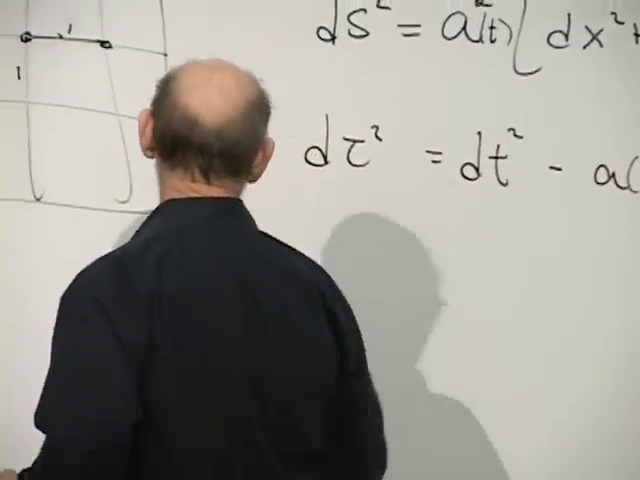
\includegraphics[width=0.62\textwidth]{lecture_02_figure_02.png}
\caption{동행 좌표 격자 스케치와 시간에 따라 변하는 스케일 인자를 포함한 시공간 간격.}
\end{figure}

그림이 요점을 잘 보여 줍니다. 앨리스와 밥은 동행 좌표계에서 계속 한 단위만큼 떨어져 있지만, 그 좌표 한 단위가 나타내는 미터 거리는 시간이 흐를수록 커집니다. 과거 어느 시점에 \(a(t)\)가 0이었다면 모든 물리적 거리가 0이었을 것입니다. 모든 것이 서로 위에 눌려 포개져 있었을 것입니다. 그래서 \(a\to 0\)는 무한 밀도에 해당합니다. \(a\)가 커질수록 우주는 점점 더 희박해집니다.

이 계량 형태가 모든 좌표계에서 성립하는 것은 아닙니다. 은하들과 함께 움직이는 좌표계에서 성립하는 형태입니다.

\begin{classroomqa}
\audiencequestion{그 방정식의 작은 \(t\), \(a(t)\)에서 \(t\)는 누구의 시간인가요?}\lecturetimestamp{00:19:19}
\lecturerresponse{은하들과 함께 움직이는 시계가 측정하는 시간입니다. 같은 우주 시계 공장에서 만든 똑같은 시계를 은하에 실어 보낸다고 상상해 보세요. 이 좌표계에서 시간 변수는 그 시계들이 측정하는 바로 그 시간입니다. 은하의 세계선에서는 고유 시간이 이 좌표 시간과 같습니다.}
\end{classroomqa}

실제로 동행하는 은하의 세계선을 따라가면,
\begin{equation}
dx=dy=dz=0,
\end{equation}
따라서
\begin{equation}
d\tau^2 = dt^2,
\end{equation}
이고, 그러므로
\begin{equation}
dt=d\tau.
\end{equation}

\begin{classroomqa}
\audiencequestion{이 계량 형태를 불변으로 유지하는 변환이 있나요?}\lecturetimestamp{00:23:08}
\lecturerresponse{회전은 그렇습니다. \(dx^2+dy^2+dz^2\)가 회전에 대해 불변이기 때문입니다. 하지만 로런츠 부스트는 이 형태를 보존하지 않습니다. 물질 자체가 은하들과 함께 움직이는 좌표계를 정하며, 다른 좌표계에서는 우주가 등방적으로 보이지 않을 것입니다.}
\end{classroomqa}

\section{중력장 속 발사체}

뉴턴 역학을 우주 전체에 적용하기 전에 한 걸음 물러나 더 간단한 문제부터 살펴보면 좋습니다. 큰 질량 \(M\), 그보다 훨씬 작은 질량 \(m\), 그리고 처음에 바깥쪽으로 주는 충격량이 있습니다. 충격량을 받은 뒤 작은 질량은 중력장 속에서 움직이며 뉴턴 역학이 예측하는 대로 운동합니다.

우주론 논의에서 중요한 것은 전체 궤도 문제가 아닙니다. 중요한 것은 에너지 보존입니다. 운동 에너지는
\begin{equation}
\frac{1}{2}mv^2.
\end{equation}

\begin{figure}
\centering
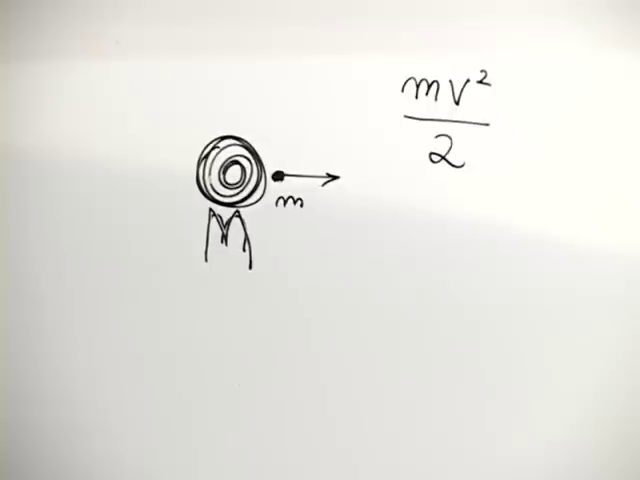
\includegraphics[width=0.42\textwidth]{lecture_02_figure_03.png}
\caption{바깥쪽으로 움직이는 시험 질량과 운동 에너지 항 \(\frac{1}{2}mv^2\).}
\end{figure}

중력 퍼텐셜 에너지에는 두 질량의 곱과 뉴턴 상수가 들어가며, 분모에는 거리의 1승이 들어갑니다. 칠판에 쓴 식에서는 인자들이 \(mMG/D\)의 순서로 나옵니다. 그러므로 여기서도 그 순서를 유지하는 편이 좋습니다.
\begin{equation}
-\frac{mMG}{D}.
\end{equation}
따라서 전체 에너지는
\begin{equation}
\frac{1}{2}mv^2-\frac{mMG}{D}.
\end{equation}
에너지 보존 법칙은 논의 중인 특정 입자에 대해 이 양이 시간에 따라 변하지 않는다는 것만 말해 줍니다. 입자마다 에너지는 다를 수 있습니다.

\begin{figure}
\centering
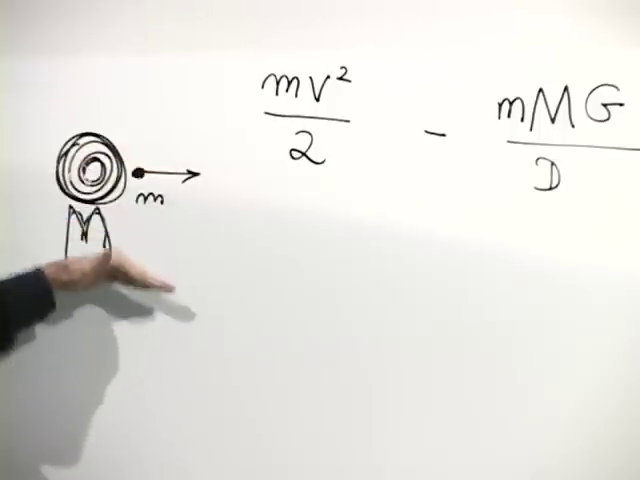
\includegraphics[width=0.62\textwidth]{lecture_02_figure_04.png}
\caption{반지름 방향으로 움직이는 시험 질량의 전체 뉴턴 에너지: 운동 에너지 항에서 중력 퍼텐셜을 뺀 값.}
\end{figure}

음의 부호가 중요합니다. 중력은 인력이므로 중력 퍼텐셜 에너지는 음수입니다. 입자를 더 가까이 가져오면 음의 퍼텐셜 에너지의 크기가 커집니다. 입자를 더 멀리 옮기면 퍼텐셜 에너지는 덜 음수가 됩니다.

\begin{classroomqa}
\audiencequestion{거리에 따라 퍼텐셜 에너지가 감소하는 게 아니라 증가하나요?}\lecturetimestamp{00:34:13}
\lecturerresponse{그렇습니다. 상수는 잠시 잊고 \(1/D\)와 \(-1/D\)의 그래프를 보세요. 힘은 퍼텐셜 에너지가 감소하는 쪽으로 작용합니다. 그러므로 인력은 위아래가 뒤집힌 곡선 \(-1/D\)에 해당합니다. 따라서 입자가 안쪽으로 움직일수록 퍼텐셜 에너지는 거리에 따라 증가하고 더 음수가 됩니다.}
\end{classroomqa}

\begin{figure}
\centering
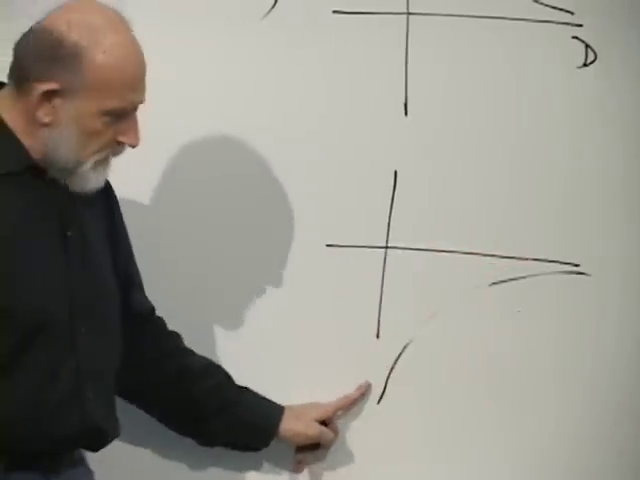
\includegraphics[width=0.46\textwidth]{lecture_02_figure_05.png}
\caption{중력 퍼텐셜 에너지의 부호를 설명하는 \(1/D\)와 \(-1/D\)의 정성적 비교.}
\end{figure}

\section{탈출 속도}

이제 가능한 경우를 분류해 봅시다. 에너지는 양수, 음수 또는 0일 수 있습니다. 경우는 이 세 가지뿐입니다.

\begin{itemize}
\item 에너지가 음수이면 입자는 속박되어 있다. 입자를 위로 던졌을 때 속도가 너무 작으면 입자는 올라가다가 느려지고, 방향을 바꾸어 다시 떨어진다.
\item 에너지가 양수이면 입자는 탈출한다. 중력은 처음에는 입자의 속도를 줄이지만 멈추게 할 정도는 아니며, 결국 입자는 영이 아닌 점근적 바깥쪽 속도로 멀어진다.
\item 에너지가 정확히 영이면 입자는 탈출 속도로 움직인다. 이는 탈출하는 경우와 탈출하지 못하는 경우 사이의 경계 사례다.
\end{itemize}

초기 속도가 충분히 작으면 처음부터 퍼텐셜 항이 우세하여 에너지가 음수입니다.

\begin{figure}
\centering
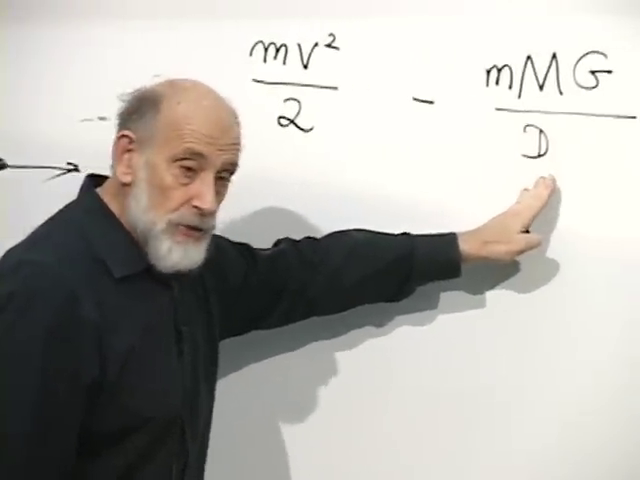
\includegraphics[width=0.62\textwidth]{lecture_02_figure_06.png}
\caption{작은 바깥쪽 속도에서는 음의 퍼텐셜 항이 전체 에너지를 좌우한다.}
\end{figure}

에너지가 0인 경우 거리는 계속 커지지만 속도는 계속 줄어듭니다. 입자는 유한한 시간 안에 정지할 수 없습니다. 만약 정지한다면 다시 안쪽으로 떨어질 것입니다. 따라서 거리는 상한 없이 커지는 반면 속도는 0에 가까워집니다.

우주론에서 중요한 직접적인 비유가 바로 이것입니다. 우주도 같은 방식으로 거동할 수 있습니다. 초기의 바깥쪽 허블 흐름이 충분히 크면 모든 것이 서로를 벗어나 멀어집니다. 너무 작으면 중력이 이겨 우주는 거대한 수축에 이릅니다. 탈출 속도와 정확히 유사한 경계 사례도 있습니다.

\section{뉴턴 정리}

우주론 문제를 단순화할 수 있는 것은 역제곱 법칙에 관한 뉴턴 정리 덕분입니다.

물질이 어떤 중심을 기준으로 구대칭 분포를 이룬다면, 분포 바깥에 있는 입자가 받는 중력은 모든 질량이 중심에 모여 있는 경우와 정확히 같습니다. 하지만 정리는 그보다 더 강한 내용을 담고 있습니다. 입자가 분포 안에 있으면 더 작은 반지름 안쪽의 질량만 기여합니다. 더 큰 반지름에 있는 질량은 알짜 힘을 만들지 않습니다.

정리를 가장 깔끔하게 보여 주는 경우는 얇은 구각입니다. 완전한 구형 껍질은 중심에서 벗어난 곳을 포함해 그 내부 어디에 있는 입자에도 중력을 전혀 가하지 않습니다. 처음에는 놀라운 결과처럼 보이지만 \(1/r^2\) 법칙에서는 사실입니다.

\begin{classroomqa}
\audiencequestion{방금 든 예에서 입자가 경계를 가로지를 때 힘이 불연속적으로 변하는 것처럼 보이는데, 이를 조금 의아하게 여겨야 하지 않을까요?}\lecturetimestamp{00:48:19}
\lecturerresponse{그렇습니다.
이상적인 무한히 얇은 껍질이라면 놀라운 일이며, \(1/r^2\) 힘 법칙에서만 나타나는 특성입니다.
실제 껍질에는 두께가 있으므로 변화가 매끄럽게 이어지지만, 이상적인 껍질에 관한 이 명확한 진술이 바로 뉴턴 정리의 놀라운 성질입니다.}
\end{classroomqa}

그림을 보면 이 정리가 그럴듯하게 느껴집니다. 점질량을 물의 점원으로 바꾸어 생각해 봅시다. 3차원에서는 바깥쪽 흐름이 \(1/r^2\)처럼 감소합니다. 이런 점원들을 구형 껍질을 따라 연속적으로 배치해 보세요. 껍질 바깥에서는 모든 물이 중심에 모여 있는 것과 흐름이 정확히 같습니다. 껍질 안에는 중심에 원천이 없으므로 알짜 흐름이 있을 수 없습니다. 중력 정리의 바탕에도 같은 구조가 있습니다.

여기서 요점은 정리를 다시 유도하는 것이 아니라 활용하는 것입니다.

\section{균질한 우주를 하나의 물체 문제로 보기}

이제 우주론으로 돌아갑시다. 은하가 균일한 기체처럼 채워진 작은 우주 영역을 생각해 봅시다. 원한다면 그 중심에 자신을 둘 수 있습니다. 이는 편의를 위한 선택일 뿐입니다. 누구나 자신을 중심에 있다고 정할 수 있고, 어느 경우든 같은 방정식이 나와야 합니다.

동행 좌표 \(x\)에서 \(x\)축 위에 있는 은하 하나를 고릅니다. 우주는 등방적이므로 어떤 축을 택해도 상관없습니다. \(x=0\)를 중심으로 하고 그 은하를 지나는 구를 그립니다. 뉴턴 정리에 따르면 그 은하가 받는 힘은 구 안의 모든 질량이 중심에 모여 있고 바깥의 모든 물질은 전혀 기여하지 않는 경우와 정확히 같습니다.

이 구는 은하들과 함께 팽창합니다. 물리적 반지름은 시간에 따라 변하지만, 구 안에는 늘 같은 은하가 들어 있으므로 전체 질량도 일정합니다.

따라서 그 은하의 운동은 발사체 문제와 정확히 같은 형태의 에너지 방정식을 따릅니다.
\begin{equation}
\frac{1}{2}mv^2-\frac{mMG}{D}=\text{constant}.
\end{equation}
여기서 \(M\)은 이제 예비 그림에서의 중심 질량이 아니라 팽창하는 구 안의 질량을 뜻합니다. 그런 다음 \(2\)을 곱하고 \(m\)로 나누면 대수식이 간단해집니다. 상수를 \(m\)로 나누어도 여전히 상수이므로 다음과 같이 쓸 수 있습니다.
\begin{equation}
v^2-\frac{2MG}{D}=\text{constant}.
\end{equation}
여기서도 ``상수''란 해당 은하에 대해 시간에 따라 일정하다는 뜻입니다.

이제 스케일 인자와 연결해 봅시다. 은하까지의 물리적 거리는
\begin{equation}
D=ax,
\end{equation}
입니다. \(x\)는 고정된 동행 좌표이기 때문입니다. 속도는
\begin{equation}
v=\dot D=\dot a\,x.
\end{equation}

구 안의 질량은 밀도와 부피의 곱입니다. \(\rho\)가 질량 밀도라면,
\begin{equation}
M=\frac{4\pi}{3}\rho D^3=\frac{4\pi}{3}\rho a^3x^3.
\end{equation}
이를 에너지 방정식에 대입하면
\begin{equation}
\dot a^2x^2-\frac{2G}{ax}\left(\frac{4\pi}{3}\rho a^3x^3\right)=\text{constant},
\end{equation}
또는
\begin{equation}
\dot a^2x^2-\frac{8\pi G}{3}\rho a^2x^2=\text{constant}.
\end{equation}

좌변의 두 항은 모두 \(x^2\)에 비례합니다. 그 밖의 것은 모두 어디서나 같습니다. 따라서 우변 역시 \(x^2\)에 비례해야 합니다. 이를 상수라고 부르는 것과 모순되지 않습니다. 고정된 \(x\)마다 시간에 대해서는 일정하지만, 은하에 따라 \(x^2\)에 비례해 달라질 수 있다는 뜻입니다. 이는 자연스럽습니다. 더 멀리 있는 은하일수록 더 빠르게 움직이기 때문입니다.

그러므로 공통 인자인 \(x^2\)를 나눠 없앱니다. 이제 남은 상수는 시간과 공간 모두에 무관합니다. 역사적으로 표준적인 방식에 따라 이를 \(-k\)로 씁니다.
\begin{equation}
\dot a^2-\frac{8\pi G}{3}\rho a^2=-k.
\end{equation}
\(a^2\)로 나누면,
\begin{equation}
\left(\frac{\dot a}{a}\right)^2=\frac{8\pi G}{3}\rho-\frac{k}{a^2}.
\end{equation}

이것이 유명한 프리드만-로버트슨-워커 방정식입니다. 다만 강의에서는 사실상 프리드만의 방정식이라고도 덧붙입니다. 부호 규약은 역사적인 것입니다. \(-k\)라고 쓴다고 해서 \(k\)가 반드시 양수여야 하는 것은 아닙니다. \(k\)는 양수, 음수 또는 0일 수 있습니다. 광속을 \(1\)으로 놓는 단위계에서 \(k\)는 무차원입니다.

\section{밀도와 물질 지배 방정식}

다음 질문은 바로 이것입니다. \(\rho\)는 무엇일까요? 이것은 상수가 아닙니다. 우주가 팽창하면 밀도는 감소합니다.

이러한 의존성을 나타내기 위해 좌표 공간에서 한 변의 길이가 각각 \(x\), \(y\), \(z\) 단위인 정육면체를 생각해 봅시다. 좌표와 함께 정육면체도 팽창하므로 그 안에는 언제나 같은 은하들이 들어 있습니다. 따라서 그 좌표 정육면체 안의 질량은 일정합니다.

\editorialnote{강의에서는 여러 단계에서 기호 \(M\)를 다시 사용합니다. 여기서는 앞서 나온 중심 질량 및 구 안의 질량과 구별하기 위해 단위 좌표 정육면체 안의 질량을 \(M_{\Box}\)로 표기합니다.}

정육면체의 물리적 한 변 길이는 \(a\)이므로 물리적 부피는 \(a^3\)입니다. 따라서
\begin{equation}
\rho=\frac{M_{\Box}}{a^3}.
\end{equation}
이것이 물질 지배 경우입니다. 우변에는 보통의 비상대론적 물질의 밀도만 들어 있습니다.

\begin{classroomqa}
\audiencequestion{이 방정식에 따르면 허블 상수는 \(\rho\)의 함수입니다. 그러면 상수가 아니네요.}\lecturetimestamp{01:19:21}
\lecturerresponse{맞습니다. 허블 상수는 상수가 아닙니다. 밀도에 의존하고, 밀도는 시간에 따라 변합니다. 강의에서는 기말시험 문제가 하나뿐이라면 이런 질문이 될 수 있다고 농담하기도 합니다. 허블 상수는 상수인가?}
\end{classroomqa}

\(\rho=M_{\Box}/a^3\)를 프리드만 방정식에 대입하면
\begin{equation}
\left(\frac{\dot a}{a}\right)^2=\frac{8\pi G M_{\Box}}{3a^3}-\frac{k}{a^2}.
\end{equation}

이제 임의로 정한 값들이 무엇인지 분명해졌습니다. 단위 좌표 정육면체 안의 질량과 \(k\)의 값이 필요합니다. \(k\)의 세 가지 부호는 발사체 문제의 세 가지 에너지 경우에 대응합니다.

\begin{itemize}
\item \(-k>0\)이면 에너지는 사실상 탈출 속도보다 높고, 우주는 영원히 팽창한다.
\item \(-k<0\)이면 중력이 결국 우세해져 우주는 다시 수축한다.
\item \(k=0\)이면 우주는 정확히 탈출 속도에 해당하는 상태다.
\end{itemize}

\begin{classroomqa}
\audiencequestion{\(k=0\)인가요? 그러면 두 은하 사이의 속도는 0에 가까워지나요?}\lecturetimestamp{01:21:12}
\lecturerresponse{그렇습니다. 임계 경우에는 속도가 0에 가까워지지만 거리는 여전히 상한 없이 커집니다. 은하들은 계속 멀어지되 그 속도가 점점 더 느려집니다. 유한한 시간 안에 실제로 정지한다면 다시 안쪽으로 떨어질 것입니다.}
\end{classroomqa}

\section{임계 경우 \(k=0\)}

이제 가장 간단한 경우인 \(k=0\)를 택합시다. 정확히 탈출 속도에 해당하는 경우이며, 수학이 더 간단하다는 이유로만 풀이가 단순해집니다. 방정식은 다음과 같습니다.
\begin{equation}
\left(\frac{\dot a}{a}\right)^2=\frac{8\pi G M_{\Box}}{3a^3}.
\end{equation}

우변은 항상 양수이고 0이 되지 않습니다. 따라서 \(\dot a/a\)는 0을 통과할 수 없습니다. 이 경우 우주는 방향을 바꿀 수 없습니다. 항상 팽창하거나 항상 수축합니다. 팽창하는 가지를 택합시다.

이제 거듭제곱 법칙을 가정해 봅시다.
\begin{equation}
a(t)=ct^p.
\end{equation}
그러면
\begin{equation}
\dot a = cp\,t^{p-1},
\end{equation}
따라서
\begin{equation}
\frac{\dot a}{a}=\frac{p}{t}.
\end{equation}
이를 미분 방정식에 대입하면
\begin{equation}
\frac{p^2}{t^2}=\frac{8\pi G M_{\Box}}{3c^3t^{3p}}.
\end{equation}
\(t\)의 거듭제곱이 서로 일치하려면 다음이 성립해야 합니다.
\begin{equation}
3p=2.
\end{equation}
그러므로
\begin{equation}
p=\frac{2}{3}.
\end{equation}
이제 상수들이 만족해야 하는 조건은
\begin{equation}
\frac{4}{9}=\frac{8\pi G M_{\Box}}{3c^3},
\end{equation}
따라서
\begin{equation}
c^3=6\pi G M_{\Box}.
\end{equation}
결과적으로
\begin{equation}
a(t)=\left(6\pi G M_{\Box}\right)^{1/3}t^{2/3}.
\end{equation}

시간을 더하는 상수는 여전히 넣을 수 있습니다. \(t\)를 \(t-t_0\)로 바꾸면 그 효과가 반영됩니다. \(a=0\)가 \(t=0\)일 때가 시간의 원점이 되도록 정하면, 남아 있던 상수는 사라집니다.

따라서 우주의 팽창은 시간에 따라 다음과 같이 변한다.
\begin{equation}
a(t)\propto t^{2/3}.
\end{equation}
시간에 따라 선형적으로 팽창하지는 않는다.
선형적인 증가는 가속되지 않는 운동에 해당한다.
여기서는 팽창이 느려진다.

이 공식을 \(t=0\)까지 거슬러 적용하면 스케일 인자는 0으로 가고 밀도는 무한대로 발산합니다. \(a=0\)라고 말하는 것은 극단적인 표현입니다. 물질이 너무 높은 밀도에 이르면 어떻게 되는지 우리는 알지 못합니다. 핵심은 초기 어느 단계에 모든 것이 매우 빽빽하게 모여 원자, 원자핵, 쿼크가 모두 비정상적으로 높은 밀도의 상태에 함께 있었다는 것입니다.

\section{허블 상수와 우주의 나이}

임계 모형에서는
\begin{equation}
H(t)=\frac{\dot a}{a}=\frac{2}{3t}.
\end{equation}
따라서 허블 상수는 우주의 나이의 역수에 대략 비례합니다.
\begin{equation}
t=\frac{2}{3H}.
\end{equation}
이것이 계산의 주요 성과 가운데 하나입니다. 현재의 허블 상수를 측정하면 우주의 나이를 추정할 수 있습니다. 적어도 뉴턴 모형이 더는 타당하지 않게 되는 시점까지의 나이를 얻습니다.

제시된 우주의 나이는 대략 \(13\)억 년에서 \(14\)억 년 사이입니다. 또한 본문은 \(k=0\)가 관측과 매우 잘 맞는다고 말합니다. 거기서 제시한 정밀도 수준에서는 \(k=0\)에서 유의미하게 벗어난다는 사실이 알려져 있지 않습니다.

\begin{classroomqa}
\audiencequestion{\(M\)와 \(a\)가 무엇인지 조금 헷갈립니다.}\lecturetimestamp{01:39:16}
\lecturerresponse{둘 다 격자를 어떻게 선택하느냐에 따른 임의성이 있습니다. 기준 상자의 크기를 바꾸면 그 안에 든 물질의 양이 달라지고 스케일 인자의 수치도 달라집니다. 물리적으로 의미 있는 양은 밀도 \(M/a^3\) 또는 격자 선택에 의존하지 않는 \(a/M^{1/3}\) 같은 조합입니다. \(k=0\) 해에서는 \(t^{2/3}\)에 곱해지는 미지의 상수가 \(\dot a/a\)에서 상쇄되므로, 나이 관계식 \(t=2/3H\)은 기준 상자의 질량에 의존하지 않습니다.}
\end{classroomqa}

해에서 그 상쇄는 즉시 확인할 수 있습니다. 만약
\begin{equation}
a(t)=Ct^{2/3},
\end{equation}
라면
\begin{equation}
\dot a=\frac{2}{3}Ct^{-1/3},
\end{equation}
그러므로
\begin{equation}
\frac{\dot a}{a}=\frac{2}{3t}.
\end{equation}
상수 \(C\)는 완전히 소거됩니다.

\section{뉴턴 역학에 의한 유도가 성립하는 이유}

강의 후반부에 이르면 뉴턴 역학에 의한 유도가 상대론적 유도와 왜 이토록 잘 일치하는가라는 질문이 제기됩니다.

\begin{classroomqa}
\audiencequestion{이 모든 것은 열린 우주라는 가정에 의존하는 것 같습니다.}\lecturetimestamp{01:45:44}
\lecturerresponse{이 단계의 유도는 뉴턴 역학에 기반하며, 뉴턴 물리학은 평탄한 공간을 전제로 합니다. 공간의 기하학으로 \(k\)를 해석하는 문제는 다음 강의로 미룹니다. 다음 강의에서는 \(k=0\)가 평탄한 공간에 해당하고, 다른 부호들은 곡률이 있는 공간 기하와 연결됩니다.}
\end{classroomqa}

\begin{classroomqa}
\audiencequestion{아주 오래전에는 미터 자의 길이가 \(a\)에 의존했나요?}\lecturetimestamp{01:47:53}
\lecturerresponse{훨씬 더 과거로 거슬러 가면 물질이 너무 빽빽하게 모여 있어 서로 분리된 미터 자가 실제로 존재하지 않았을 것입니다. 그보다 이전에는 미터 자들이 서로 압착되었을 것입니다. 강의에서는 상대론이 완벽하게 강체인 물체도 허용하지 않는다고 덧붙입니다. 물체가 완벽한 강체라면 한쪽을 밀었을 때 그 신호가 빛보다 빠른 순간적인 속도로 반대쪽에 전달되어야 합니다.}
\end{classroomqa}

\begin{classroomqa}
\audiencequestion{뉴턴 역학과 상대론에서 이런 방정식의 일치가 나타나는 이유는 무엇이라고 생각하시나요?}\lecturetimestamp{01:49:03}
\lecturerresponse{뉴턴 역학을 충분히 작은 영역에만 적용하고 있기 때문입니다. 그 영역이 우주 전체의 곡률 반지름에 비해 작고, 그 안의 국소 허블 속도가 광속보다 훨씬 낮다면 뉴턴 역학은 좋은 근사입니다. 강의에서는 이를 지구에서 풀의 성장을 연구하는 경우와 비교합니다. 지구 전체의 곡률을 고려하지 않고도 국소적인 현상을 이해할 수 있습니다.}
\end{classroomqa}

이것이 국소 영역에 관한 논리입니다. 뉴턴 역학은 첫째, 당면한 문제에서 공간의 곡률이 중요하지 않고, 둘째, 국소적으로 광속에 가까운 속도로 움직이는 것이 없다고 가정합니다. 우주론에서는 균질하다고 볼 수 있을 만큼 충분히 크면서도 곡률 효과를 무시할 수 있고 허블 속도가 비상대론적 범위에 머무를 만큼 충분히 작은 영역을 택한다는 뜻입니다.

이 점을 염두에 두면 뉴턴 역학의 계산은 우연히 맞아떨어진 것이 아닙니다. 상대론적 형태로도 해석할 수 있는 방정식의 국소 근사입니다. 곡률 항을 좌변으로 옮기면 프리드만 방정식은 다음과 같습니다.
\begin{equation}
\left(\frac{\dot a}{a}\right)^2+\frac{k}{a^2}=\frac{8\pi G}{3}\rho.
\end{equation}
좌변은 스케일 인자와 다음 강의에서 다룰 공간의 곡률을 포함하는 기하학적 항입니다. 우변은 에너지 밀도입니다. 이는 일반 상대성 이론에서 기대할 수 있는 바로 그런 형태의 방정식입니다.

다음 시간에는 곡률 자체와 아인슈타인 방정식, 그리고 상대론적 유도와 뉴턴 역학에 의한 유도의 관계를 살펴보겠습니다.
